\documentclass{article}
\usepackage{booktabs}
\usepackage{amsthm, amssymb, amsmath}
\usepackage{mathtools}
\usepackage{graphicx}
\usepackage{algorithm}
\usepackage{algorithmic}

\usepackage{todonotes}

\usepackage{stmaryrd, color, tikz, dsfont}
\usepackage{booktabs}

\DeclareMathOperator*{\argmax}{arg\,max}
\DeclareMathOperator*{\argmin}{arg\,min}

\newcommand{\bn}{{\sc bn}}
\newcommand{\bdn}{{\sc bdn}}
\newcommand{\Pa}{\mathit{Pa}}
\renewcommand{\dag}{{\sc dag}}
\newcommand{\holderFig}[1]{\missingfigure[figwidth=\linewidth, figheight=6cm]{{#1}}}
\newcommand{\ra}[1]{\renewcommand{\arraystretch}{#1}}


\newtheorem{theorem}{Theorem}
\newtheorem{lemma}{Lemma}

% Recommended, but optional, packages for figures and better typesetting:
\usepackage{microtype}
\usepackage{subcaption}

% hyperref makes hyperlinks in the resulting PDF.
% If your build breaks (sometimes temporarily if a hyperlink spans a page)
% please comment out the following usepackage line and replace
% \usepackage{icml2018} with \usepackage[nohyperref]{icml2018} above.
\usepackage{hyperref}

% Attempt to make hyperref and algorithmic work together better:
\newcommand{\theHalgorithm}{\arabic{algorithm}}

% Use the following line for the initial blind version submitted for review:
\usepackage{icml2019}
\begin{document}	
	\twocolumn[
	\icmltitle{Learning Structured Decision Problems with Unawareness}
		
	\begin{icmlauthorlist}
		\icmlauthor{Craig Innes}{ed}
		\icmlauthor{Alex Lascarides}{ed}
	\end{icmlauthorlist}
	
	\icmlaffiliation{ed}{Institute for Language Cognition and Computation, University of Edinburgh, Edinburgh, Scotland}

	
	\icmlcorrespondingauthor{Craig Innes}{craig.innes@ed.ac.uk}
	\icmlcorrespondingauthor{Alex Lascarides}{alex@inf.ed.ac.uk}
	
	% You may provide any keywords that you
	% find helpful for describing your paper; these are used to populate
	% the "keywords" metadata in the PDF but will not be shown in the document
	\icmlkeywords{}
	
	\vskip 0.3in
	]
	
	% this must go after the closing bracket ] following \twocolumn[ ...
	
	% This command actually creates the footnote in the first column
	% listing the affiliations and the copyright notice.
	% The command takes one argument, which is text to display at the start of the footnote.
	% The \icmlEqualContribution command is standard text for equal contribution.
	% Remove it (just {}) if you do not need this facility.
	
	\printAffiliationsAndNotice{}  % leave blank if no need to mention equal contribution
	
	\begin{abstract}
		Structured models of decision making often assume an agent is aware of all possible states and actions in advance. This assumption is sometimes untenable. In this paper, we learn bayesian decision networks from both domain exploration and expert assertions in a way which guarantees convergence to optimal behaviour, even when the agent starts unaware of actions or belief variables that are critical to success. Our experiments show that our agent learns optimal behaviour on small and large decision problems, and that allowing an agent to conserve information upon discovering new possibilities results in faster convergence.
	\end{abstract}
	
	\section{Introduction}
	\label{sec:introduction}
	Probabilistic graphical models have proven useful in representing richly-structured decision tasks \cite{koller_probabilistic_2009}. Many techniques exist to learn a model's structure and parameters from experience \cite{tsamardinos_max-min_2006,bartlett_integer_2017} and expert advice \cite{masegosa_interactive_2013}. Unfortunately, all such methods assume the way the domain is \emph{conceptualized}---the belief and action variables used to describe the problem---is completely known in advance. Often, this assumption does not hold.
	
	In medicine, for example, suppose an agent prescribes a drug, but later a senior pharmacologist objects to the prescription based on a reason unforeseen by the agent---the patient carries a newly discovered genetic trait, and the drug produces harmful side effects in its carriers. Further, this discovery may occur after the agent has already learned a lot about how other (foreseen) factors impact the drug's effectiveness. As \citet{coenen_asking_2017} point out, such scenarios are common in human discussion---the answer to a question may not only provide information about which of the questioner's existing hypotheses are likely, but also reveal unforeseen hypotheses not yet considered. This example also shows that while it may be infeasible for an agent to gather all relevant factors of a problem \emph{before} learning, it may be  easy for an expert to offer contextually relevant advice \emph{during} learning. Another example is in robotic skill learning. Methods like \citet{cakmak_designing_2012} enable an expert to teach a robot \emph{how} to perform a new action, but not \emph{when} to use it. In lifelong learning scenarios, we want to integrate new skills into existing decision problems without forcing the robot to restart learning each time.
	
	Current learning and decision making models don't address these issues; they assume the task is to use data to \emph{refine} a distribution over a \emph{fixed} hypothesis space. Under this framework, any change to the set of possible hypotheses constitutes an unrelated problem. The above examples, however, illustrate a sort of \emph{reverse bayesianism} \cite{karni_reverse_2013}, where the hypothesis space itself expands over time.
	
	Rather than \emph{overcoming} unawareness of states and actions, we could instead represent unawareness as an infinite number of hidden variables \cite{wood_non-parametric_2006}, or abandon learning a structured model and use densely connected hidden layers to implicitly learn structure from raw sensory input \cite{mnih_human-level_2015}. Both these approaches have drawbacks. First, neither currently address how to adapt what one has learned when a new \emph{action} is discovered. More importantly, the hidden layers/variables are not tied to grounded concepts with explicit meaning, so an agent cannot easily justify its decisions to a user, or articulate the limits of its current understanding to solicit help from others.
	
	We instead propose an agent which explicitly overcomes its unawareness, and constructs an interpretable model of the problem. This paper makes three contributions: First, an algorithm which incrementally learns \emph{all} components of a decision problem as a Bayesian Decision Network (\bdn{}). This includes the reward function and probabilistic dependencies between variables, but also the \emph{set of belief and action variables themselves} (Sections \ref{sec:full-awareness-learn}, \ref{sec:adapting}). Second, an agent-expert communication protocol (Section \ref{sec:expert-guidance}) which \emph{interleaves} contextual advice with learning, and guarantees our agent converges to optimal behaviour despite starting unaware of factors critical to success. Third, experiments on decision tasks of varying sizes showing our agent successfully learns optimal behaviour in practice (Section \ref{sec:experiments}).
		
	\section{Learning with Full Awareness}
	\label{sec:full-awareness-learn}
		
	We focus on learning observable, single-stage decision problems with discrete states and actions. In this paper, we learn optimal behaviour by learning a \emph{bayesian decision network} (a bayesian network extended with actions and rewards), which defines the optimal policy. We start with the scenario where the agent is aware of all possible states and actions, then address the task where the agent is \emph{unaware} of relevant states and actions.

	
	\subsection{Making Optimal Decisions}
	\label{sec:optimal-decisions}
	Our agent's goal is to learn the policy $\pi^*$ which, given evidence $e$, chooses the action $a$ which maximizes its \emph{expected utility} $EU(a | e) = \sum_{s'} P(s' | a, e) \mathcal{R}(s')$ across all states $s'$. If $P(s | a, e)$ or reward function $\mathcal{R}$ are unknown, the agent must learn them via trial and error. Our agent balances \emph{exploiting} its current estimate of $\pi^*$ with \emph{exploring} the domain by using an \emph{$\epsilon$-greedy policy} (one which acts randomly with probability $\epsilon > 0$, and according to the current estimate of $\pi^*$ with probability $1 - \epsilon$). For any policy $\pi$, we can measure the expected loss in reward against the true optimal policy $\pi_+$ using (\ref{eqn:policy-error})---the \emph{policy error}.
	
	\begin{equation}
	\label{eqn:policy-error}
	PE(\pi) = \sum_e P(e) \left(EU(\pi_+(e) | e) - EU(\pi(e) | e)\right)
	\end{equation}
	
	If there are many states, evaluating the expected utility directly is infeasible. The next sections show how to exploit a problem's inherent structure to make computations tractable.
	
	\subsection{Bayesian Networks}
	\label{sec:bns}
	
	Bayesian networks (\bn{}s) decompose the state space of the problem into a set of belief variables $\mathcal{X} = \{ X_1, \dots X_n \}$. Each state is $s$ a joint assignment to all variables in $\mathcal{X}$ (i.e., $s \in v(\mathcal{X})$). An \bn{} is a directed acyclic graph (\dag) $\Pa$ and parameters $\theta$ which exploit the conditional independencies between variables in $\mathcal{X}$. For each $X \in \mathcal{X}$, $\Pa_X \in \Pa$ is the \emph{parent set} of $X$. Given $Pa_X$, the value of $X$ is conditionally independent of all $Y \in \mathcal{X} \setminus \Pa_X$ which are non-descendants of $X$. The parameters $\theta_X \in \theta$ then define the conditional probability distributions $\theta_X = P(X | \Pa_X)$.
	
	Given $\mathcal{X}$, we can learn the most likely structure $\Pa^*$ and parameters $\theta^*$ from observed data $D_{0:t} = [d_0, \dots, d_t]$ (where $d_i \in v(\mathcal{X})$) by learning $P(\Pa | D_{0:t})$ and $P(\theta | D_{0:t}, \Pa)$. A common way to calculate $P(\Pa | D_{0:t})$ is to use the \emph{Bayesian Dirichlet Score} (BD-Score) \citep{heckerman_learning_1995}:
		
	\begin{align}
	\label{eqn:struct-posterior}
	&P(\Pa | D_{0:t}) \propto \prod_{X \in \mathcal{X}} \textsc{BD}_t(X, Pa_X)
	\end{align}
	
	\begin{align}
		\label{eqn:fam-score}
		&\textsc{BD}_t(X, Pa_X) = \nonumber\\
		&\quad P(\Pa_X) \prod_{\mathclap{j \in v(\Pa_X)}} \frac{\beta(N^t_{0|j} + \alpha_{0|j}, \dots , N^t_{m | j} + \alpha_{m | j})}{\beta(\alpha_{0 | j}, \dots, \alpha_{m|j})}
	\end{align}
	
	Here, $\beta(n_1, \dots, n_m)$ is the \emph{multivariate beta function}, and $N^t_{X=i|\Pa_X=j}$ is the number of states in $D_{0:t}$ where $X$ has assignment $i$ and its parents have joint assignment $j$.\footnote{Where the context is clear, we compress this notation to $N^t_{i|j}$} The $\alpha_{i|j}$ parameters come from the dirichlet priors over $\theta$ and act as a ``pseudo-count'' when data is sparse. We typically choose the prior $P(\Pa)$ to penalize complex structures, as in equation (\ref{eqn:struct-prior}) which assigns a cost of $\rho < 0.5$ for each extra parent:
	
	\begin{equation}
	\label{eqn:struct-prior}
	P(\Pa_X) = \rho^{|\Pa_X|} (1 - \rho)^{|\mathcal{X} \setminus \Pa_X|}
	\end{equation}
	
	Unfortunately, evaluating the full posterior of (\ref{eqn:struct-posterior}), or even finding its maximum, is infeasible for even a moderate number of variables, as the number of possible \bn{}s is hyper-exponential in the size of $\mathcal{X}$ \cite{tian_computing_2009}. To tackle this, most methods approximate $\Pa^*$ via either local search \cite{teyssier_ordering-based_2005}, sampling methods \cite{madigan_bayesian_1995}, or by reducing the search space of structures considered reasonable \cite{buntine_theory_1991}. For our task, we have another issue---most \bn{} learning methods operate \emph{once} on a single \emph{batch} of data, and thus consider the collection of \emph{sufficient statistics} (i.e., the BD-scores of each $\Pa_X$ and their associated $N_{i|j}$) to be a negligible pre-computed cost. In a decision problem, agents gather data \emph{incrementally} and exploit their current beliefs during learning, so we must \emph{update} the sufficient statistics each time step.
	
	To address these issues, we follow \citet{buntine_theory_1991} by constructing a \emph{reasonable parent lattice} $\mathcal{P}_X$ for each $X$. Figure \ref{fig:buntine-lattice} shows an example lattice for $X_1$. Starting from $\emptyset$, we construct larger parent sets by combining sets seen so far,and track the highest scoring set according to (\ref{eqn:fam-score}). Any parent-set with a score lower than some proportion $\kappa$ of the best score, is considered ``unreasonable'', and is not expanded further.\footnote{In contrast to \citet{buntine_theory_1991} we also consider all subsets of a reasonable parent set to be reasonable.}
		
	Once we have our reduced set $\mathcal{P}_X$ for each $X$, we can find the combination of reasonable parent sets which maximize (\ref{eqn:struct-posterior}) and form a valid \dag{}. In our task we will be learning $\mathcal{X}$, so cannot assume we know a total-ordering $\prec$ over $\mathcal{X}$ (as \citet{buntine_theory_1991} does), and thus cannot choose each $Pa_X^*$ independently. Instead, following \citet{bartlett_integer_2017}, we treat finding $\Pa^*$ as the linear program given below:
	
	\begin{equation}
	\begin{array}{rrllcl}
	\displaystyle \max & \multicolumn{3}{l}{\sum\limits_{X \in \mathcal{X}}\sum\limits_{\Pa_X \in \mathcal{P}_X} I(\Pa_X \rightarrow X) \ln[BD(X, \Pa_X)] } \\
	\textrm{s.t.} & \sum\limits_{\Pa_X \in \mathcal{P}_X} &I(\Pa_X \rightarrow X) = 1 & \forall X \\
	&\sum\limits_{\substack{X \in C \\ \Pa_X \cap C = \emptyset}} &I(\Pa_X \rightarrow X) \geq 1 & \forall C \subseteq \mathcal{X}\\
	&&I(\Pa_X \rightarrow X) \in \{0, 1\} & \forall X, \Pa_X\\
	\end{array}
	\label{eqn:ilp}
	\end{equation}
	
	The variables $I(\Pa_X \rightarrow X)$ denote whether we chose $\Pa_X$ as $X$'s parent set, while the constraints ensure each $X$ has only one parent set and that the parent sets form a \dag{}.
	
	\begin{figure}
		\centering
		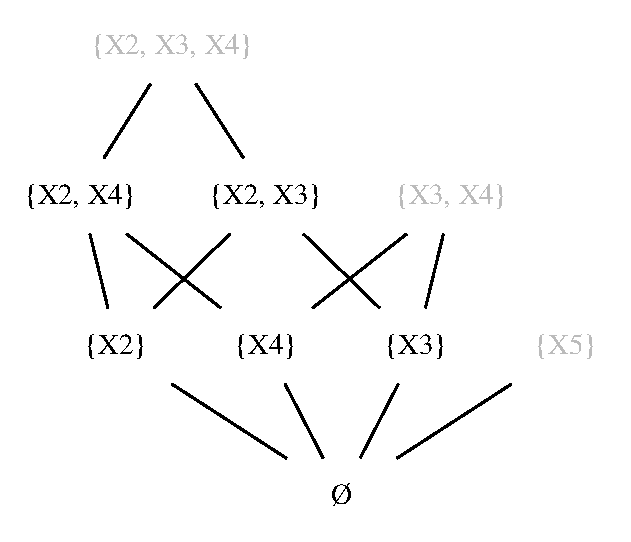
\includegraphics[width=0.5\linewidth]{buntineLattice}
		\caption{Parent lattice for $X_1$. Grey nodes are unreasonable}
		\label{fig:buntine-lattice}
	\end{figure}
		
	Once we have learned the most likely structure $\Pa^*$, we can learn its most likely parameters $\theta^*$ via (\ref{eqn:expected-params}):
	
	\begin{equation}
	\label{eqn:expected-params}
	\begin{aligned}
	\mathbb{E}_{\theta | D_{0:t}, \Pa} (\theta_{i | j}) = \frac{N_{i | j} + \alpha_{i | j}}{N_{. | j} + \alpha_{. | j}}
	\end{aligned}
	\end{equation}
	
	Our method has three main advantages. First, reducing the number of reasonable parent sets and using the modular $BD$-score means we can \emph{incrementally} update the probability of each $Pa_X$ using past calculations of (\ref{eqn:fam-score}) via (\ref{eqn:incremental-struct-score}):\footnote{We include a proof of (\ref{eqn:incremental-struct-score}) in the technical supplement.}
	
	\begin{equation}
	\label{eqn:incremental-struct-score}
	\textsc{BD}_{t}(X, \Pa_X) = \textsc{BD}_{t-1}(X, \Pa_X) \frac{N^{t}_{i|j} + \alpha_{i | j} - 1}{N^{t}_{.|j} + \alpha_{.|j} - 1}
	\end{equation}
	
	Second, expressing structure learning as a linear program makes it easy to add \emph{extra} structural constraints later (as we do in section \ref{sec:expert-guidance}). Third, each lattice $\mathcal{P}_X$ implicitly captures an \emph{approximate distribution} over each $X$'s parents.\footnote{Technically, without $\prec$, each $\mathcal{P}_X$ is a distribution over \emph{markov blankets} for $X$, but we enforce acyclicity, so this is not an issue.} In section \ref{sec:adapting}, the agent uses this distribution to conserve information as its awareness of $\mathcal{X}$ expands.
	
	\subsection{Learning to Act with Bayesian Decision Networks}
	A \bdn{} \cite{russell_artificial_2002} is a \bn{} augmented with actions and rewards. It is a tuple $\langle \mathcal{A}, \mathcal{X}, \mathcal{R}, Pa, \theta \rangle$. Here, $\mathcal{A} = \{ A_1, \dots , A_m \}$ are the \emph{action variables} the agent controls (where a full action $a$ is a member of  $v(\mathcal{A})$). As before, $\mathcal{X}$ are the belief variables, but they are now partitioned into $\mathcal{X} = \mathcal{B} \cup \mathcal{O}$, where $\mathcal{B}$ is the set of variables the agent observes \emph{before} taking action, and $\mathcal{O}$ are the variables which describe the \emph{outcome} of that action. The reward function $\mathcal{R} : v(scope(\mathcal{R})) \rightarrow \mathds{R}$ gives the reward received for each state, where $scope(\mathcal{R}) \subseteq \mathcal{X}$ are the variables which determine the reward. While $\Pa$ and $\theta$ still describe the probabilistic dependencies, each $\Pa_X$ can now include belief \emph{and} action variables (i.e., $\forall X, \Pa_X \subset \mathcal{X} \cup \mathcal{A}$). A \emph{domain trial} at time $t$ is a tuple $d_t = \langle s_t, a_t, r_t \rangle$, where $s_t = \langle b_t, o_t \rangle$, $b_t \in v(\mathcal{B})$, $o_t \in v(\mathcal{O})$, $a_t \in v(\mathcal{A})$ and $r_t = \mathcal{R}(s_t)$. 
		
	Figure \ref{fig:bdn-example} shows an example \bdn{}. Here, the agent chooses assignments for action variables {\sc Topical Cream} and {\sc Oral Drug } based on observing { \sc Gene X}, then receives a reward based on outcomes { \sc Disease}, and {\sc Side Effects}. We note that \bdn{}s are essentially a subset of the notation used for \emph{influence diagrams} \cite{howard_influence_2005}. Influence diagrams add \emph{information arcs} from belief variables to action variables, which show the variables in $\mathcal{B}$ that the agent observes before choosing values for each $A \in \mathcal{A}$. For simplicity of explanation, we omit information arcs, and instead assume all action variables are set simultaneously, with access to observations of all variables in $\mathcal{B}$.
	
	\begin{figure}
		\centering
		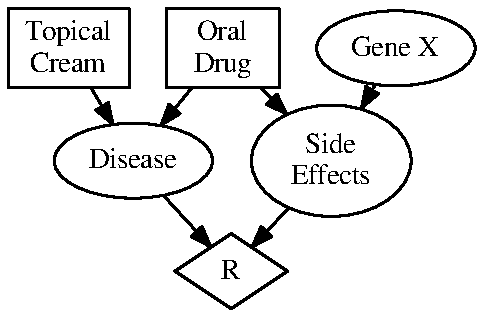
\includegraphics[width=0.5\linewidth]{dnMedicine}
		\caption{\bdn{} for medical example. Rectangles are action variables, ovals are belief variables, and diamonds are reward nodes}
		\label{fig:bdn-example}
	\end{figure}

	We can use the same techniques from section \ref{sec:bns} to learn $\Pa^*$ and $\theta^*$ for \bdn{}s. Similarly, we can learn reward function $\mathcal{R}_t$ from $scope(\mathcal{R})$, and $D_{0:t}$ by setting $\mathcal{R}_t(s_t[scope(\mathcal{R})]) = r_t$,\footnote{Here, $s[\mathcal{Y}]$ projects assignment $s$ over the variables in $\mathcal{Y}$.} and by defaulting to indifference for unseen states (e.g., by setting the reward of unseen states to 0). Given a learned \bdn{}, the agent then chooses a policy $\pi^*$ which maximizes the expected utility from section \ref{sec:optimal-decisions} (where $a \in v(\mathcal{A})$ and $e \in v(\mathcal{B})$).
	
	\section{Overcoming Unawareness}	
	So far, we've assumed our agent was aware of all relevant variables in $\mathcal{X} \cup \mathcal{A}$ and all members of $scope(\mathcal{R})$. We now drop this assumption. From here onward we denote the true set of belief variables, actions, and reward scope as $\mathcal{X}^+$, $A^+$ and $scope_+(\mathcal{R})$, and the learner's awareness of them at time $t$ as  $\mathcal{X}^t$, $A^t$, and $scope_t(\mathcal{R})$.
	
	Suppose $X^+ = \{ X_1, X_2\}$, $X^0 = \{ X_1 \}$, $\mathcal{A}^+ = \{ A_1, A_2 \}$, $\mathcal{A}^t = \{ A_1 \}$. We assume the agent can't observe the value of variables it is unaware of. In the medical example from section \ref{sec:introduction}, if $X_2$ is particular gene, we assume the agent cannot detect the presence of that gene if it is unaware it exists. We also assume the agent cannot perform actions it is unaware of (i.e., if the agent is unaware of variable $A_2$ then it cannot set it to a value other than its default value).\footnote{This assumption, while reasonable, may not always hold (E.g., an agent may lean on a button while unaware it is part of the task).} This means at time $t=0$, the agent does not observe the true trial $d_0$, but rather $\langle s_0[\mathcal{X}^0], a_0[\mathcal{A}^0], r_0 \rangle$. But awareness of those missing factors may be crucial to learning $\pi_+$. For example, the best action may depend upon whether $X_2$ is true, or the optimal policy may sometimes involve setting $A_2$ to a value other than its default. The next sections thus answer two main questions. First, how can an agent discover and overcome its own unawareness by asking for help? Second, when an agent discovers a new variable, how can they integrate it into their current model while conserving what they have learned from past experience?

	\subsection{Expert Guidance}
	\label{sec:expert-guidance}
	Our agent can expand its awareness via advice from an expert. Teacher-apprentice learning is common in the real world, as it allows learners to receive contextually relevant advice which may inform them of unforeseen concepts.
	
	This paper assumes the expert is cooperative and infallible. Further, we abstract away the complexity of grounding natural language statements in a formal semantics and instead assume that the agent and expert communicate via a pre-specified formal language (though see e.g., \cite{zettlemoyer_online_2007} for work on this problem). We do not, however, assume the expert knows the \emph{agent's} beliefs about the \bdn{}. The variables $\mathcal{X}^e$ and $\mathcal{A}^e$ express the expert's knowledge of our agent's awareness, and include only those actions  the expert has explicitly seen the agent perform, or variables the agent mentions in conversation.
	
	As argued in the introduction, the goal is to provide a minimal set of communicative acts so that interaction between the agent and expert mirrors human teacher-apprentice interaction. Concretely, this means we want our system to have two properties. First, the expert should mostly allow the agent to learn by themselves, interjecting only when the agent performs sufficiently poorly, or when they explicitly ask a question. Second, our expert should be able to give \emph{non-exhaustive} answers to queries. This is because, in practice, it is unlikely a human expert will be able to give exhaustive answers to all questions due to either cognitive bounds or a lack of information. Following the maxims of \citet{grice_logic_1975}, a cooperative speaker should give answers which provide just enough information to resolve the agent's current dilemma. The next sections identify four advice types, whose combination guarantee the agent eventually behaves optimally, regardless of initial awareness.
	\subsubsection{Better Action Advice}
	
	If the expert sees the agent perform a sub-optimal action, it can tell the agent a better action to take instead. For example: ``When it is raining, take your umbrella instead of your sun hat''. Our goal is to avoid interrupting the agent every time it makes a mistake, so we specify the following conditions for when the agent performs poorly enough to warrant correction: Let $t$ be the current time step, and $t'$ be the time the expert last uttered advice. When (\ref{eqn:last-spoken-interval}-\ref{eqn:minimal-action}) hold:
	
	\begin{gather}
	\label{eqn:last-spoken-interval}
	t-t' > \mu \\
	\label{eqn:suboptimal-performance}
	\sum_{t' \leq i \leq t} \frac{EU(\pi_+(b_i) | b_i) - EU(a_i | b_i)}{t - t'} > \beta \\
	\label{eqn:reward-below-expected}
	EU(a_t|b_t) \geq r_t \\
	\label{eqn:better-action-available}
	\exists \mathcal{A}',a' \in v(\mathcal{A}^e \cup \mathcal{A}'), EU(a' | b_t) > EU(a_t | b_t) \\
	\label{eqn:minimal-action}
	\begin{aligned}
	\nexists \mathcal{A}^{''}, (&a'' \in v(\mathcal{A}^e \cup \mathcal{A}''), EU(a{''} | b_t) > E(a_t | b_t) \\
	\wedge\ &|\mathcal{A}''| < |\mathcal{A}'|)
	\end{aligned}
	\end{gather}
	
	Then the expert will utter advice of the form (\ref{eqn:better-action-utterance}):
	
	\begin{equation}
	\label{eqn:better-action-utterance}
	EU(a' | w^b_t) > EU(a_t[\mathcal{A}^t \cup \mathcal{A}'] | w^b_t)
	\end{equation}
	
	Equation (\ref{eqn:last-spoken-interval}) ensures some minimum time $\mu$ has passed since the expert last gave advice, while (\ref{eqn:suboptimal-performance}) ensures the expert won't interrupt unless its estimate of the agent's policy error is above some threshold $\beta$. Together, $\mu$ and $\beta$ define how \emph{tolerant} the expert will be to the agent's poor performance before deciding to give advice. Equation (\ref{eqn:reward-below-expected}) ensures that the expert's suggested action has an expected reward higher than what the agent received at time $t$. Finally, (\ref{eqn:better-action-available}-\ref{eqn:minimal-action}) ensure not only that a better action $a'$ exists,  but also that $a'$ introduces the minimum amount of potentially unforeseen action variables $\mathcal{A}'$ needed to improve the agent's behaviour. This means there isn't another action $a''$ which could be advised while revealing fewer unaware variables to the agent. This follows from our desire to give non-exhaustive advice, by first suggesting improvements which use concepts the agent is already aware of, rather than introducing many new action variables all at once.
	
	Equation (\ref{eqn:better-action-utterance})---the expert's utterance---requires explanation. On first thought, the expert should utter $EU(a' | b_t) > EU(a_{t} | b_t)$, thus fully describing $b_t$. But remember that the agent's awareness $\mathcal{B}^t$ may be a tiny subset of $\mathcal{B}^+$. Uttering such advice may involve revealing many variables the agent is currently unaware of. This is exactly the type of cognitively-taxing exhaustive explanation we wish to avoid. Conversely, restricting the description to $\mathcal{X}^e$ could make the advice false: there may exist a $b' \neq b_t$ where $b'[\mathcal{X}^e] = b_t[\mathcal{X}^e]$, but $EU(a_t | b') > EU(a' | b')$. The answer is to use an \emph{ambiguous term} $w^b$, whose \emph{intended} meaning is the true state $b$ (i.e $\llbracket w^b \rrbracket \in v(\mathcal{B}^+)$), but whose \emph{default} interpretation by the agent is $b[\mathcal{B}^t]$. In words, the expert says \emph{``In the last step, $a'$ would have been better than $a_t$''}.
	
	By introducing ambiguity, the agent can now interpret (\ref{eqn:better-action-utterance}) in two ways. The first is as a \emph{partial description} of the true \bdn{}, which is true \emph{regardless} of what it learns in future. On hearing (\ref{eqn:better-action-utterance}), the agent adds (\ref{eqn:action-relevant}-\ref{eqn:better-reward-exists}) to its knowledge:
	
	\begin{align}
	\label{eqn:action-relevant}
	&\forall A \in \mathcal{A}', A \in \mathcal{A}^+ \wedge \exists X \in scope_+(\mathcal{R}), anc(A, X) \\
	\label{eqn:better-reward-exists}
	&\exists s \in v(\mathcal{X}^+), s[\mathcal{B}^t] = s_t[\mathcal{B}^t] \wedge \mathcal{R}_+(s) > r_t
	\end{align}
		
	Where $anc(X,Y)$ means $X$ is the ancestor of $Y$ (i.e., there is a directed path from $X$ to $Y$ in the true \bdn{}). Equations (\ref{eqn:action-relevant}-\ref{eqn:better-reward-exists}) imply that any variable the expert utters must be \emph{relevant} to the problem. In other words, it must exert influence on at least one variable in $scope_+(\mathcal{R})$, and that there exists some state the agent could have reached which would yield a better reward than the one it got. In fact, we can enforce all equations of the form (\ref{eqn:action-relevant}) when learning $\Pa^*$ by adding the constraint (\ref{eqn:relevance-constraint}) to our linear program:
	
	\begin{equation}
	\label{eqn:relevance-constraint}
	\forall Y \notin scope(\mathcal{R}):\quad \sum_{\mathclap{\substack{X \in \mathcal{X} \\ \Pa_X : Y \in \Pa_X}}} I(\Pa_X \rightarrow X) \geq 1
	\end{equation} 
		
	The second way the agent could use (\ref{eqn:better-action-utterance}) is by adding its \emph{default interpretation} of the advice to its current knowledge:

	\begin{equation}
	\label{eqn:better-action-defeasible}
	\forall b \in \mathcal{B}^+: b[\mathcal{B}^t] = b_t[\mathcal{B}^t] \Rightarrow EU(a' | b) > EU(a | b)
	\end{equation}
	
	The agent can then enforce (\ref{eqn:better-action-defeasible}) by choosing $a'$ whenever $b[\mathcal{B}^t] = b_t[\mathcal{B}^t]$, regardless of what seems likely from $D_{0:t}$. We should now see that even with a cooperative, infallible expert, even abstracting away issues of grounding natural language, misunderstandings can still happen due to differences in agent and expert awareness. As the next section shows, such misunderstandings can reveal gaps in the agent's awareness and help to articulate queries whose answers guarantee the agent expands its awareness.
	
	Lemma \ref{thm:action-awareness} guarantees the expert's advice strategy continues to reveal unforeseen actions to the agent so long as its performance in trials exceeds the expert's tolerance.\footnote{We include proofs of all lemmas in the technical supplement}
	
	\begin{lemma}
		\label{thm:action-awareness}
		Consider an agent with awareness $A^t \subset A^+$, and expert following (\ref{eqn:last-spoken-interval}-\ref{eqn:better-action-utterance}). As $k \rightarrow \infty$, either $PE(\pi_{t+k}) \rightarrow c \leq \beta$ or the expert utters (\ref{eqn:better-action-utterance}) where $\mathcal{A}' \neq \emptyset$.
	\end{lemma}	
	
	\subsubsection{Resolving a Misunderstanding}
	
		We noted before that the agent's default interpretation of (\ref{eqn:better-action-utterance}) could lead it to misunderstand the expert's intended meaning. To illustrate, suppose the agent receives advice (\ref{eqn:advice-conflict-1}) and (\ref{eqn:advice-conflict-2}) at times $t -k$ and $t$:
		
		\begin{gather}
		\label{eqn:advice-conflict-1}
		EU(a | w^b_{t - k}) > EU(a' | w^b_{t-k}) \\
		\label{eqn:advice-conflict-2}
		EU(a | w^b_{t}) < EU(a' | w^b_{t})
		\end{gather}
		
		While the intended meaning of each statement is true, the agent's default interpretations of $w^s_{t-k}$ and $w^s_{t}$ may be identical. That is, $b_{t-k}[\mathcal{B}^t] = b_{t}[\mathcal{B}^t]$. From the agent's perspective, (\ref{eqn:advice-conflict-1}) and (\ref{eqn:advice-conflict-2}) conflict, and thus give the agent a clue that its current awareness of $\mathcal{X}^+$ is deficient. To resolve this conflict, the agent asks (\ref{eqn:misunderstanding-q}) (in words, \emph{``which $B$ has distinct values in $b_{t-k}$ and $b_t$?''}) and receives an answer which provides monotonic information of the form (\ref{eqn:misunderstanding-a-anc}):
		
		\begin{gather}
		\label{eqn:misunderstanding-q}
		?\lambda B(B\in \mathcal{B}^+ \wedge s_{t - k}[B] \neq s_{t}[B]) \\
		\label{eqn:misunderstanding-a-anc}
		B' \in \mathcal{B}^+ \wedge \exists X \in scope_+(\mathcal{R}), anc(B', X)
		\end{gather}
		
		Notice there may be many variables in $\mathcal{B}^+ \setminus \mathcal{B}^t$ whose assignments differ in $b_{t-k}$ and $b_t$. Thus, the expert's answer can be \emph{non-exhaustive}. This means the agent must abandon its previous defeasible interpretations of the form (\ref{eqn:better-action-defeasible}), but can keep (\ref{eqn:action-relevant}-\ref{eqn:better-reward-exists}), as these are true regardless of what the true \bdn{} is. Lemma \ref{theorem:state-space-awareness} guarantees the expert will reveal new belief variables provided misunderstandings can still arise.
		
		\begin{lemma}
			\label{theorem:state-space-awareness}
			Consider an agent with awareness $\mathcal{X}^t \subset \mathcal{X}^+$, $\mathcal{A}^t = \mathcal{A}^+$. If $\exists b', \exists b \neq b', b[\mathcal{B}^t] = b'[\mathcal{B}^t]$ and $\pi_+(b) \neq \pi_+(b')$, then as $k \rightarrow \infty$, either $PE(\pi_{t+k}) \rightarrow c \leq \beta$, or the expert utters (\ref{eqn:misunderstanding-a-anc}) such that $B' \notin \mathcal{B}^t$
		\end{lemma}
	\subsubsection{Unforeseen Rewards}
	
	In typical \bdn{}s (where we assume the agent starts fully aware of $\mathcal{X}^+, A^+$, and $scope_+(\mathcal{R})$), we tend only to think of the trials as providing \emph{counts}. For an unaware agent, a trial $d_t = \langle s_t, a_t, r_t \rangle$ also encodes \emph{monotonic information}:
	
	\begin{equation}
	\label{eqn:trial-monotonic}
	\exists s, s[\mathcal{X}^t] = s_{t}[\mathcal{X}^t] \wedge \mathcal{R}_+(s) = r_{t}
	\end{equation}
	
	This, along with (\ref{eqn:better-reward-exists}), constrain the form of $\mathcal{R}$ the agent can learn. Recall that $scope_t(\mathcal{R})$ may be only a subset of $scope_+(\mathcal{R})$, so it might be impossible to construct an $\mathcal{R} : v(scope_t(\mathcal{R})) \rightarrow \mathds{R}$ satisfying all descriptions (\ref{eqn:trial-monotonic}) gathered so far. Further, those extra variables in $scope_+(\mathcal{R}) \setminus scope_t(\mathcal{R})$ may not be in $\mathcal{X}^t$. To resolve this, if the agent fails to construct a valid $\mathcal{R}$, it asks (\ref{eqn:unforeseen-reward-q}) (in words, \emph{``which variable $X$ (that I don't already know) is in $scope(\mathcal{R})$?''}), receiving an answer of the form (\ref{eqn:unforeseen-reward-monotonic}):
	
	\begin{gather}
	\label{eqn:unforeseen-reward-q}
	?\lambda X(X\in \mathit{scope}_+(\mathcal{R}) \bigwedge_{\mathclap{X'\in scope_t(\mathcal{R})}}
	X\neq X') \\
	\label{eqn:unforeseen-reward-monotonic}
	X'' \in scope_+(\mathcal{R}) \wedge X'' \in \mathcal{X}^+
	\end{gather}
	
	Again (\ref{eqn:unforeseen-reward-monotonic}) may be \emph{non-exhaustive}. Even so, we can guarantee that the agent's reward function eventually equals $\mathcal{R}_+$.
	
	\begin{lemma}
		\label{thm:reward-scope-awareness}
		Consider an $\epsilon$-greedy agent with awareness $\mathcal{A}^t = \mathcal{A}^+$, $scope_t(\mathcal{R}) \subseteq scope_+(\mathcal{R})$. As $k \rightarrow \infty$, there exists a $K$ such that $\forall s, \forall k \geq K$, $\mathcal{R}_{t+k}(s) = \mathcal{R}_{+}(s)$.
	\end{lemma}
	
	\subsubsection{Unknown effect}
	
	Recall that, to keep the problem tractable, our agent searches for \bdn{}s in the space of ``reasonable'' parent sets $\mathcal{P}$. Unfortunately, there might be no valid \bdn{} within $\mathcal{P}$ which also satisfies the constraints of the form (\ref{eqn:relevance-constraint}). The most obvious case of this is when a variable $X \notin scope_t(\mathcal{R})$ has no children in \emph{any} reasonable \dag{} (i.e., $\forall Y, \forall \Pa_Y \in \mathcal{P}_Y, X \notin \Pa_Y$). Here, the agent can ask \emph{why} $X$ is relevant by asking (\ref{eqn:unknown-effect-question}) (\emph{``what $V$ does $X$ affect directly?''}). The answer (e.g., $X \in \Pa_{V'}$) imparts information (\ref{eqn:unknown-effect-a:anc}) to the agent:
	
	\begin{gather}
	\label{eqn:unknown-effect-question}
	? \lambda V (X \in \Pa_V) \\
	\label{eqn:unknown-effect-a:anc}
	V' \in \mathcal{X}^+ \wedge \exists Y \in scope_+(\mathcal{R}), anc(V', Y)
	\end{gather}
	
	\subsection{Adapting to Unforseen Factors}
	\label{sec:adapting}
	Section \ref{sec:expert-guidance} showed four ways to expand the agent's awareness of $\mathcal{X}$, $\mathcal{A}$, and $scope(\mathcal{R})$. To improve on simply restarting learning, we must now say how the agent \emph{adapts} its beliefs about $\Pa$ and $\theta$ when its awareness expands.
	
	\subsubsection{Adding a new belief variable}
			
	When the agent discovers a belief variable $Z$, its old distributions over parent sets no longer cover all possible parents. That is, for $X \in \mathcal{X}^{t-1}$, $\mathcal{P}_{X}$ did not cover cases where $Z$ was a parent of $X$. Worse, the agent \emph{cannot observe $Z$'s values in $D_{0:t}$}, so cannot observe $N^{t-k}_{Z  = i| j}$, or $N^{t-k}_{X = i | j}$ when $Z \in \Pa_X$. The $\alpha$-parameters involving $Z$ are also undefined, yet we need them to calculate $\Pa^*$ and $\theta^*$ via (\ref{eqn:expected-params}-\ref{eqn:incremental-struct-score}).
	
	Discovering a new variable makes the size of each (observed) state \emph{dynamic}, in contrast to standard problems where they are \emph{static} (e.g., $\langle X_1 = 0, X_2 = 1 \rangle$ becomes $\langle X_1 = 0, X_2 = 1, Z = ?\rangle$ ) . We could phrase this as a missing data problem: $Z$ was hidden in the past but visible in future states, so estimate missing values and structure via e.g., \emph{expectation maximization} \cite{friedman_bayesian_1998}. But such methods commit us to costly passes over the full batch of data and makes finding $\Pa^*$ for problems with more than a handful of variables intractable by eliminating the modularity of the $BD$-score. Alternatively, we could ignore states with missing information when we require counts involving $Z$. For example, we could use $P(\Pa_{X} | D_{t:n})$ to score $\Pa_{X}$ when $Z \in \Pa_{X}$ but use $P(\Pa_{X} | D_{0:n})$ when $Z \notin \Pa_{X}$. But as \citet{friedman_sequential_1997} point out, most structure scores, including (\ref{eqn:struct-posterior}), assume we evaluate models with the \emph{same data}. If we compare models using different data sets (even two sets from the same distribution), the learner favours models evaluated with the smallest data set.
	
	Instead, our method discards data $D_{0:t-1}$ gathered during the learner's old view of the hypothesis space, but conserves the \emph{posterior} probabilities learned from it to create new \emph{priors} for $\Pa$ and $\theta$ in the expanded space. On discovering the new variable $Z$, the agent updates each distribution over the parent sets $\Pa_X$ ($X \neq Z$) to cover parent sets which include $Z$. Equation (\ref{eqn:old-parent-sets-new-vocab}) creates a new prior $P'(\Pa_X)$ from the old posterior. Here, $C$ is the normalizing constant and $0 < \gamma \leq 1$ expresses how much we trust our current $\mathcal{P}$:
	
	\begin{align}
	\label{eqn:old-parent-sets-new-vocab}
	&P'(\Pa_X) = \gamma P'(\Pa_X | \mathcal{P}_X) + (1 - \gamma) P(\Pa_X)\\
	&\begin{aligned}
	&P'(\Pa_X | \mathcal{P}_X) = \\
	&\begin{cases}
	0 & \text{if } \Pa_X \notin \mathcal{P}_X \\
	\frac{(1 - \rho)}{C} \textsc{BD}_{t-1}(X, \Pa_X) & \text{if } Z \notin \Pa_X \\
	\frac{\rho}{C} \textsc{BD}_{t-1}(X, \Pa'_X) & \text{if } \Pa_X = \Pa'_X \cup \{ Z \}
	\end{cases}
	\end{aligned}
	\end{align}
		
	This update preserves the relative likelihood among the parent sets without $Z$. It also preserves our bias towards simple structures by giving only a small portion $\rho$ of the probability mass of parent sets without $Z$ to those with $Z$. This still leaves us to define a distribution over $\Pa_{Z}$ itself. The agent has no evidence on $Z$'s parents at the moment of $Z$'s discovery, so defaults to using the initial prior (\ref{eqn:struct-prior}).
	
	To adapt $\theta^*$, we return to the issue of the counts $N^t_{i | j}$ and $\alpha$-parameters. As before, we wish to avoid the complexity of estimating $Z$'s past values. Instead, we \emph{throw away} the past states $D_{0:t-1}$ and their counts $N^{t-1}_{i | j}$, but \emph{keep} the relative likelihoods they gave rise to by packing these into new $\alpha$-parameters, as shown in (\ref{eqn:param-posterior-to-prior}) ($K$ is a constant):
	
	\begin{equation}
	\label{eqn:param-posterior-to-prior}
	\begin{aligned}
	&N^t_{i | j} = 0 \text{ for all } i,j, X, \Pa_X \\
	&\alpha_{i | j} = 
	\begin{cases}
	\frac{K}{|Z|}  P(j \rvert \theta^*_{t-1}) & \text{if } X = Z \\
	\frac{K}{|Z|}  P(i, j[\Pa_X \setminus Z] \rvert \theta^*_{t-1}) & \text{if } Z \in \Pa_{X}\\
	K  P(i, j \rvert \theta^*_{t-1}) & \text{otherwise}
	\end{cases}
	\end{aligned}
	\end{equation}
	
	Equation (\ref{eqn:param-posterior-to-prior}) summarizes the counts $D_{0:t-1}$ based on inferences from the old \bdn{}, then encodes these inferences in the $\alpha$-parameters of the new parameter prior. The new $\alpha$-parameters ensure that the likelihoods inferred from past states bias the estimate of $\Pa^*$ and $\theta^*$ as more trials arrive. The larger $K$ is, the more what it learned \emph{before} discovering $Z$ influences its reasoning \emph{after} discovering $Z$.
	
	\subsubsection{Adding a new action variable}
	
	When the agent discovers a new action variable $A$, the same issue arises---the agent did not consider $A$ as a possible parent to any $X \in \mathcal{X}^{t-1}$, so must revise $\mathcal{P}$ with $A$ as a possibility. Unlike for belief variables, however, we don't need to discard $D_{0:t-1}$. Since we assume that the agent cannot influence action variables it is unaware of, we can simply fill in the default value of $A$ in all past trials $D_{0:t-1}$.
	
	\subsubsection{Expanding the reward function scope}
	Learning that a variable $X$ is in the scope of $\mathcal{R}$ may cause us to revise $\Pa^*$, even if $X \in \mathcal{X}^{t-1}$. This is because expanding $scope_t(\mathcal{R})$ loosens the constraints of the form (\ref{eqn:relevance-constraint}) which may allow us to construct a higher scoring \bdn{} structure that was previously invalid.
	
	\begin{algorithm}[t]
		\caption{Learning \bdn{}s with Unawareness}
		\label{alg:full-system}
		\begin{algorithmic}[1]
			\STATE {\bfseries Input: } $\mathcal{A}^0$, $\mathcal{X}^0$, $\Pa^0$, $\theta^0$, $\mathcal{P}^0$
			\FOR{$t=1\dots\mathit{maxTrials}$}
				\STATE $b_t$ $\gets$ Generate new state
				\STATE $\langle o_t, a_t, r_t \rangle \gets$ \textsc{$\epsilon$-greedy}($b_{t}[\mathcal{X}^t]$)
				\STATE $N^t_{i|j} \gets$ Update with $b_t[\mathcal{X}^t], o_t[\mathcal{X}^t]$
				\STATE $BD_t(X, \Pa_X) \gets$ Update via (\ref{eqn:incremental-struct-score}) for $\Pa_X \in \mathcal{P}_X$
				\IF{$t \equiv 0 \pmod \tau$}
					\STATE Revise $\mathcal{P}^t$
				\ENDIF
				\IF{Exists $X$ with no reasonable children}
					\STATE Ask (\ref{eqn:unknown-effect-question}) and update $\mathcal{X}^t$, $\mathcal{P}^t$
				\ENDIF
				\STATE $\mathcal{R}^t \gets$ Update with constraints (\ref{eqn:trial-monotonic}, \ref{eqn:better-reward-exists})
				\IF{Update to $\mathcal{R}_t$ fails}
					\STATE Ask (\ref{eqn:misunderstanding-q}) and update $scope_t(\mathcal{R}), \mathcal{X}^t, \mathcal{P}^t$
				\ENDIF
				\IF{ (\ref{eqn:last-spoken-interval}-\ref{eqn:minimal-action}) are true}
					\STATE $\mathit{actAdvice} \gets$ Expert advises (\ref{eqn:better-action-utterance})
					\STATE Update $\mathcal{A}^t$, $\mathcal{P}^t$ according to $\mathit{actAdvice}$
						\IF{$\mathit{actAdvice}$ conflicts with past utterances}
						\STATE Ask (\ref{eqn:misunderstanding-q}) and update $\mathcal{X}^t, \mathcal{P}^t$
						\ENDIF
				\ENDIF
				
				\IF{$\mathcal{X}^{t-1} \neq \mathcal{X}^t$}
					\STATE Update $N^t_{i|j}, \alpha_{i|j}, \mathcal{P}, P(\Pa)$ via (\ref{eqn:struct-prior},
					 \ref{eqn:old-parent-sets-new-vocab}, \ref{eqn:param-posterior-to-prior})
				\ENDIF
				\STATE $\langle \Pa^t, \theta^t \rangle \gets$ Solve (\ref{eqn:ilp}) (with (\ref{eqn:relevance-constraint})), and (\ref{eqn:expected-params})
				\ENDFOR
		\end{algorithmic}
	\end{algorithm}
	
	Algorithm \ref{alg:full-system} outlines the entire learning process. In most steps, the agent incrementally revises its model based on the latest trial and current reasonable parents. If enough time $\tau$ passes, or the agent's awareness expands, the agent makes larger changes to its model, including revising $\mathcal{P}$. Given algorithm \ref{alg:full-system}, theorem \ref{thm:full-unawareness-guarantee} guarantees our agent converges to a near-optimal policy, regardless of initial awareness  (provided $\mathcal{P}$ includes the true structure).
	\begin{theorem}
		\label{thm:full-unawareness-guarantee}
		Consider an agent with initial awareness $\mathcal{X}^0 \subseteq \mathcal{X}^+, A^0 \subseteq A^+ ,scope_0(\mathcal{R}) \subseteq scope_+(\mathcal{R})$ following algorithm \ref{alg:full-system} (with $\kappa = 0$). As $t \rightarrow \infty$, $PE(\pi_{t}) \rightarrow c \leq \beta$.
	\end{theorem}
			
	\section{Experiments}
	\label{sec:experiments}
	
	Our experiments show that agents following algorithm \ref{alg:full-system} converge to near-optimal behaviour not only in theory but also in practice. We also show that conserving information improves results. We do not investigate assigning explicit costs to agent-expert communication, but do show how varying the expert's tolerance affects the agent's performance.
	
	We tested agents on three randomly generated \bdn{}s of increasing size: 12, 24, and 36 variables. Our results were similar across all sizes, but the differences between agents were most pronounced on the largest case, so we present those here (Full \bdn{} specifications and results for the small and medium cases are included in the technical supplement). In each, our agent begins with minimal awareness of the true \bdn{} ($\mathcal{X}^0 = \{ O_1 \}, \mathcal{A}^0 = \{A_1\}$, $scope_0(\mathcal{R}) = \{ O_1 \}$). The agent acts in $5000$ trials, using an $\epsilon$-greedy policy ($\epsilon = 0.1$). We repeat experiments 100 times and average the results.
		
	We use the \emph{cumulative reward} across trials as our evaluation metric, which acts as a proxy for the quality of the agent's policy over time. To make the results more readable, we apply a discount of $0.99$ at each step, resulting in the metric $R^{disc}_t = r_t + 0.99 * R^{disc}_{t-1}$.
	
	\begin{figure*}
		\begin{subfigure}{0.333\textwidth}
			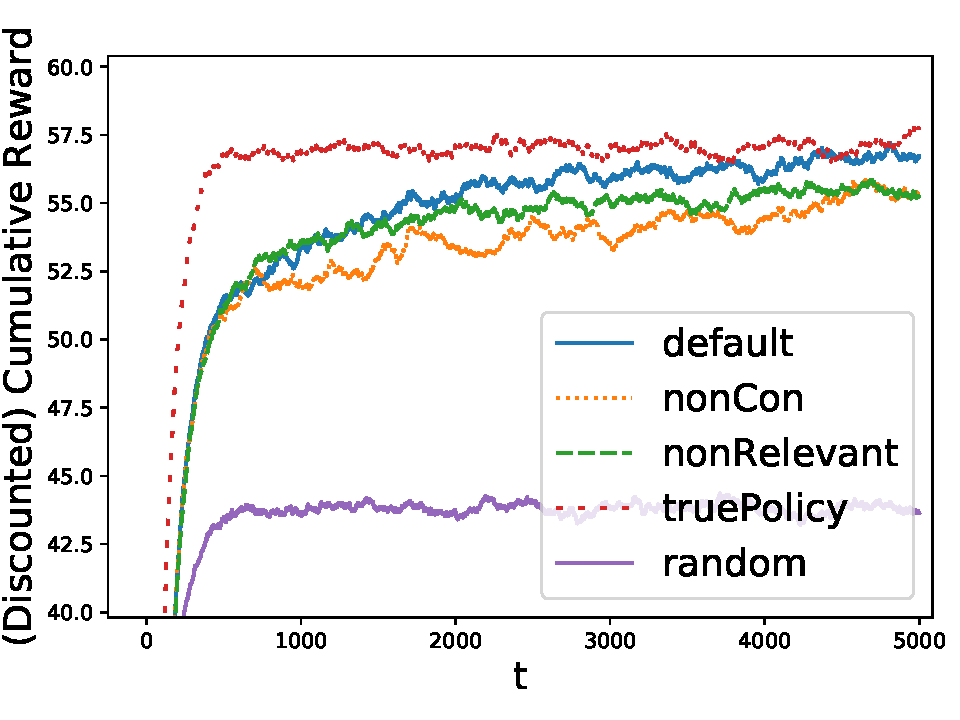
\includegraphics[width=\textwidth]{coffeeRewardsConservativity}
			\caption{}
			\label{fig:results:cons}
		\end{subfigure}
		\begin{subfigure}{0.333\textwidth}
			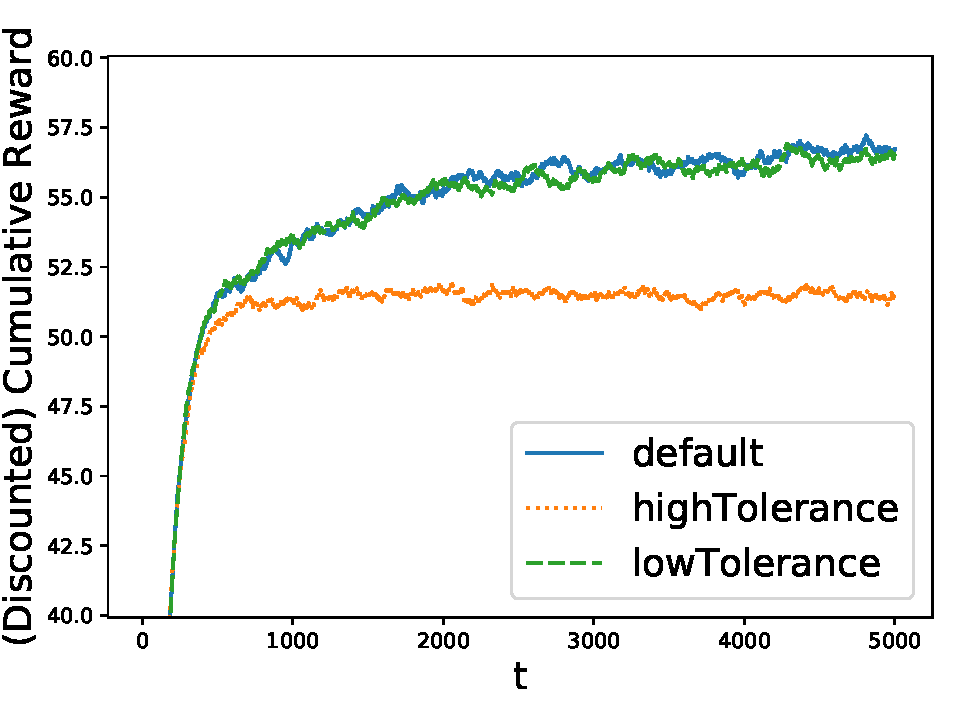
\includegraphics[width=\textwidth]{coffeeRewardsTolerance}
			\caption{}
			\label{fig:results:tol}
		\end{subfigure}
		\begin{subfigure}{0.333\textwidth}
			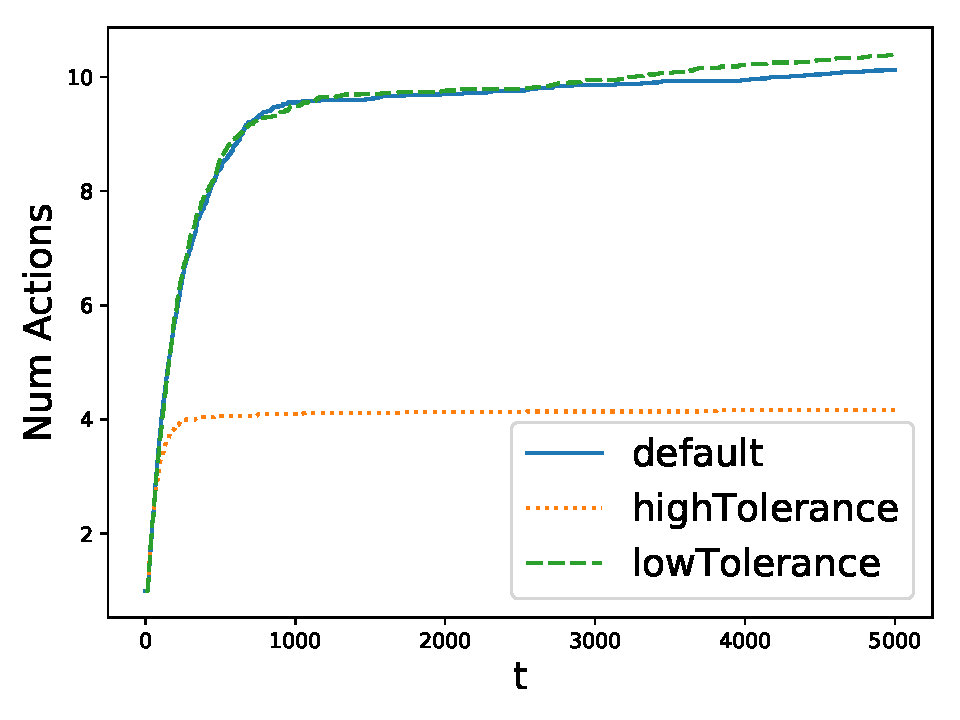
\includegraphics[width=\textwidth]{coffeeVocabSize}
			\caption{}
			\label{fig:results:vocab}
		\end{subfigure}		
		\caption{Rewards (a and b) and size of $|\mathcal{A}|$ (c) over time on the 36 variable task. Results for other tasks included in the supplement.}
		\label{fig:results}
	\end{figure*}
	
	We test several variants of our agent to show our approach is effective. The \textbf{default} agent follows algorithm \ref{alg:full-system} as is, with parameters $\kappa=0.001$, $\tau = 100$, $\rho = 0.1$, $\gamma=0.99$,  $K = 5.0$, $\mu=10$, $\beta=0.01$ in equations (\ref{eqn:struct-prior}), (\ref{eqn:last-spoken-interval}), (\ref{eqn:suboptimal-performance}), (\ref{eqn:old-parent-sets-new-vocab}), and (\ref{eqn:param-posterior-to-prior}). The \textbf{nonConservative} agent does not conserve information about $\mathcal{P}$, $\Pa$, nor $\theta$ via (\ref{eqn:old-parent-sets-new-vocab}) and (\ref{eqn:param-posterior-to-prior}) when it discovers a new factor. Instead, its discards all trials and reverts to the original prior of (\ref{eqn:struct-prior}). We include this agent to show the value of conserving information as $\mathcal{X}$ and $\mathcal{A}$ expand. The \textbf{non-relevant} agent is like the default, but does not include any constraints of the form (\ref{eqn:relevance-constraint}) when searching for $\Pa^*$. This means the agent might learn \bdn{}s where variables are completely disconnected. The \textbf{truePolicy} and \textbf{random} agents start knowing the true \bdn{}, and execute an $\epsilon$-greedy version of $\pi_+$, or choose a random action respectively. These agents give an upper/lower bound on performance. The \textbf{lowTolerance} and \textbf{highTolerance} agents change the expert's tolerance to $\beta=0.001$ and $\beta=0.1$.
	
	\subsection{Results}
	
	Across all \bdn{}s, our default agent converges to the optimal policy, despite starting unaware of factors critical to success. Figure \ref{fig:results:cons} shows the cumulative reward of the default agent compared to the non-conservative, non-relevant, true-policy and random agents. The default agent converges to the optimal policy, and does so faster than its non-conservative counterpart. This shows conserving one's beliefs on discovering new factors has value. The difference in reward compared to the non-relevant agent is smaller than expected. We suspect this is because actions which exert a strong causal influence over $scope_+(\mathcal{R})$ will be an ancestor to $scope_+(\mathcal{R})$ in $\Pa^*$ regardless of whether we enforce (\ref{eqn:relevance-constraint}). Actions the non-relevant agent leaves disconnected are those which exert little causal influence over $scope_+(\mathcal{R})$ (and thus usually have little effect on the optimal policy). This means that how much abandoning connectivity affects performance depends on how noisy the causation in the domain model is, which we don't know with certainty in advance.
	
	Figure \ref{fig:results:tol} shows how the agent's performance differs when varying the expert's tolerance level: As the tolerance increases, the agent takes longer to converge towards a good policy, and also learns a worse final policy. Figure \ref{fig:results:vocab} shows why: Early on, the agent's policy is ``good enough'' for the high tolerance expert, meaning the expert does not reveal the last few extra action variables which would net only small increases in the agent's total reward.
	
	\section{Related Literature}
	
	Models of unawareness exist in logic \cite{board_two_2011,heifetz_dynamic_2013} and game theory \cite{feinberg_games_2012}, but interpret (un)-awareness from an omniscient perspective. We instead model awareness from the \emph{agent's} perspective and offer methods to \emph{overcome} one's unawareness.
	
	\citet{rong_learning_2016} present Markov Decision Processes with Unawareness, which let an agent learn optimal behaviour even when unaware of some actions. We build on this work by providing a concrete mechanism for discovering unforeseen factors and by allowing the agent to discover \emph{explicit belief variables} rather than atomic states (which is necessary to tackle large, richly-structured problems). \citet{mccallum_reinforcement_1996} also learn an increasingly complex representation of the state space by gradually distinguishing between states which yield different rewards. Rather than dealing with unawareness, the focus of such approaches is on \emph{refining} an existing state space. In other words, they do not support introducing \emph{unforeseen} states or actions that the learner was unaware of before learning.
	
	Several works use expert interventions to correct agent behaviour \cite{torrey_teaching_2013,stone_interactively_2009}, or via agent-driven active learning \cite{masegosa_interactive_2013,murphy_active_2001}. Yet all such methods assume the expert's intended meaning can be understood without expanding the agent's conception of the state and action space. Our work allows experts to utter advice where ambiguity arises from their greater awareness of the problem.
	\section{Conclusion}
	
	We have presented an expert-assisted framework for learning structured decision problems, even when the learner starts unaware of factors critical to success. Further, our experiments show that being conservative about one's beliefs improves the effectiveness of learning. In future work, we aim to lift some assumptions imposed on the expert, and expand the range of situations in which the agent can ask for advice. For instance, we could let the expert be fallible \cite{masegosa_interactive_2013}, or leverage structural signatures \cite{elidan_discovering_2000} to guide questions asked to the expert.
	
	%\todo[inline]{Upgrade to latest 2019 style files when available. Currently using ICML 2018}
	%\todo[inline]{Check bibliography references. I think a couple looked a little incomplete!}
	
	%\missingfigure[figwidth=\linewidth, figheight=6cm, figcolor=white]{Results for connectivity test}
	
	\bibliography{thesis}
	\bibliographystyle{icml2019}
\end{document}